%%%%%%%%%%%%%%%%%%%%%%%%%%%%%%%%%%%%%%%%%%%%%%%%%%%%%%%%%%%%%%%%%%%%%%%
% Sample template for MIT Junior Lab Student Written Summaries
% Available from http://web.mit.edu/8.13/samplepaper/sample-paper.tex
%
% Last Updated June 20, 2004
%
% Adapted from the American Physical Societies REVTeK-4 Pages
% at http://publish.aps.org
%
% ADVICE TO STUDENTS: Each time you write a paper, start with this
%    template and save under a new filename.  If convenient, don't
%    erase unneeded lines, just comment them out.  Often, they
%    will be useful containers for information.
%%%%%%%%%%%%%%%%%%%%%%%%%%%%%%%%%%%%%%%%%%%%%%%%%%%%%%%%%%%%%%%%%%%%%%%


%%%%%%%%%%%%%%%%%%%%%%%%%%%%%%%%%%%%%%%%%%%%%%%%%%%%%%%%%%%%%%%%%%%%%%%
% PREAMBLE
% The preamble of a LaTeX document is the set of commands that precede
% the \begin{document} line.  It contains a \documentclass line
% to load the REVTeK-4 macro definitions and various \usepackage
% lines to load other macro packages.
%
% ADVICE TO STUDENTS: This preamble contains a suggested set of
%     class options to generate a ``Junior Lab'' look and feel that
%     facilitate quick review and feedback from one's peers, TA's
%     and section instructors.  Don't make substantial changes without
%     first consulting your section instructor.
%%%%%%%%%%%%%%%%%%%%%%%%%%%%%%%%%%%%%%%%%%%%%%%%%%%%%%%%%%%%%%%%%%%%%%%

\documentclass[aps,twocolumn,secnumarabic,nobalancelastpage,amsmath,amssymb,
nofootinbib]{revtex4}

% nofootinbib is another document class option that allows you to put
% footnotes on the page where they occur rather than at the end of the
% paper.  This makes for easier reading!

% secnumarabic is a particularly nice way of identifying sections by
% number to aid electronic review and commentary.

% amsmath and amssymb are necessary for the subequations environment
% among others

\usepackage{graphics}      % standard graphics specifications
\usepackage{graphicx}      % alternative graphics specifications
\usepackage{longtable}     % helps with long table options
\usepackage{url}           % for on-line citations
\usepackage{bm}            % special 'bold-math' package
\usepackage{subfigure}
\usepackage{booktabs}

%%%%%%%%%%%%%%%%%%%%%%%%%%%%%%%%%%%%%%%
%                                 %%%%%
% And now, begin the document...  %%%%%
%                                 %%%%%
%%%%%%%%%%%%%%%%%%%%%%%%%%%%%%%%%%%%%%%
\begin{document}
\title{Rutherford Scattering}
\author         {Kevin L. Chen. Partner: Tanooj Shah}
\affiliation    {UC Berkeley, Department of Physics}
\date{\today}

\begin{abstract}
The structure of the atom that we know today was not trivially found. It went through several iterations, from indivisible sphere to plum-pudding to orbits to quantum mechanical, with each theory backed up by the best evidence and minds of the time. This paper explores and discusses findings of the Rutherford Scattering experiment. Using a vacuum chamber, a detector, gold foil, and Americium 241, we were able to find the angular dependence of scattered alpha particles. Using the differential cross section equation, which is derived from classical scattering theory, we determined the atomic number of gold to a value of 99.77, which is within 26.3$\%$ of the actual value of 79. We also explore possible errors in our experiment such as noise and background radiation, as well as possible steps to move forward and conduct further studies to get more precise calculations for the atomic number of gold. 
\end{abstract}

\maketitle

%%%%%%%%%%%%%%%%%%%%%%%%%%%%%%%%%%%%%%%%%%%%%%%%%%%%%%%%%%%%%%%%%%%%%%%%%%%%%
\section{Introduction}

Before Rutherford, the idea of the atom underwent through various changes as more information was gained about the nature of atomic particles. The Greeks near 500 BC first began discussing the building blocks of matter, considering the possibility that there was a unit of indivisible matter, called an atom. In fact, the word ``atom'' was first coined by Greek philosophers. It was not until the early 1800s that John Dalton noticed that elements react in predictable proportions. He thus theorized that atoms were discrete, indivisible pieces of material. Later, J. J. Thomson discovered electrons through cathode ray tubes. Thomson theorized that subatomic particles form atoms through the plum pudding model (Figure~\ref{ThomsonModel}), which described the positive charge as diffuse throughout the atom, whereas the electrons are the raisins in the cake. Come 1911, and Rutherford discovers the nucleus of the atom by firing alpha particles at thin sheet of gold foil. He noticed that some alpha particles were scattered at large angles, compared to what is expected if there was a diffuse positive charge. He concluded that the atom must be made up of a concentrated nucleus and electrons orbiting around it (Figure~\ref{RutherfordModel}). In this experiment, we conduct the same experiment that Rutherford did. However, instead of a humans counting the number of hits or a fluorescent screen, we use modern technology and LabVIEW to collect data. Finally, through classical mechanics and E\&M, we can see alpha particles scattered at large angles and calculate the atomic number of gold from our data.

%%%%%%%%%%%%%%%%%%%%%%%%%%%%%%%%%%%%%%%%%%%%%%%%%%%%%%%%%%%%%%%%%%%%%%%%%%%%%
\section{Theory}
\subsection{Differential Cross Section}

To begin, the Coulomb Force facilitates the interaction between two charges. For two charges $q_1$ at $\boldsymbol{r_1}$ and $q_2$ at $\boldsymbol{r_2}$, $q_1$ will experience a force $\boldsymbol{F_1}$ described by

\begin{equation}
   \boldsymbol{F_1}={q_1q_2\over4\pi\varepsilon_0}{(\boldsymbol{r_1-r_2})\over|\boldsymbol{r_1-r_2}|^3}
   \label{Discrete Coulomb}
\end{equation}

We can find a more specific description of the Coulomb force for the Thomson Model. In the Thomson Model, the positive charge is diffusely spread throughout the atom. For instance, a particle $q$ at position $\boldsymbol{r}$ in a continuous distribution of charge will experience $\boldsymbol{F}$ given by

\begin{equation}
   \boldsymbol{F} = {q\over 4\pi\varepsilon_0}\int dq' {\boldsymbol{r} - \boldsymbol{r'} \over |\boldsymbol{r} - \boldsymbol{r'}|^3}.
   \label{Continuous Coulomb}
\end{equation}

where $dq' = \rho(\boldsymbol{r'})\,dV'$ and where the integral is taken over the volume of the atom.

\begin{figure}[hh]
  \begin{center}
    \subfigure[Thomson Model]{\label{ThomsonModel}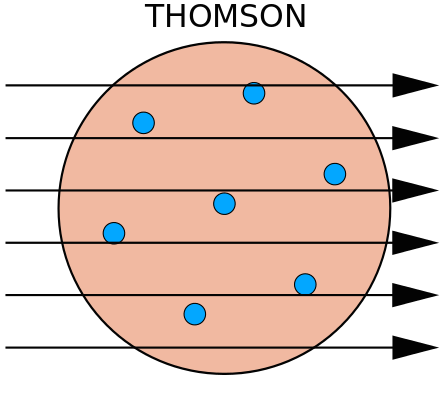
\includegraphics[width=4 cm]{Thomsonmodel.png}} 
    \subfigure[Rutherford Model]{\label{RutherfordModel}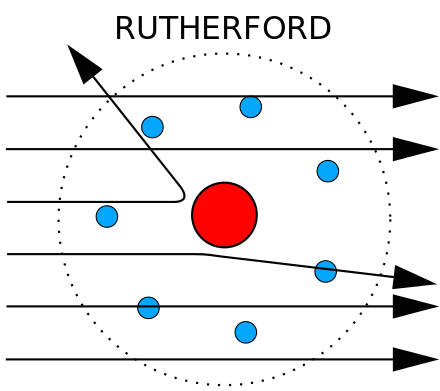
\includegraphics[width=4 cm]{rutherfordmodel.png}}\\
  \end{center}
  \caption{Comparison of two theories of the atom}[\footnotesize{``Atoms.'' Wikipedia. Wikimedia Foundation, n.d. Web. 12 Mar. 2015}]
  \label{models}
\end{figure}

Since the charge will be distributed over the entire atom, then $\rho$ will be much smaller compared to if all the charge was concentrated in a smaller area. In fact, the nucleus has been shown to be on the order 100,000 times smaller than the atom itself (for example, the factor is 23,000 for uranium and 145,000 for hydrogen).

In this experiment, we observe that some alpha particles do in fact experience a very large deflection when passing through gold foil, indicative of a strong Coulomb Force. This strong Coulomb Force must come from a concentration of positive charge, which can be described by Equation~\ref{Discrete Coulomb} rather than Equation~\ref{Continuous Coulomb} if the size of the alpha particle is comparable to the size of the nucleus. 

In this experiment, we are trying to determine the charge of the gold nucleus. In order to do this, we must consider the fraction of particles that scatter as a function of the angle. In Reference~\cite{Melissinos}, A.C. Melissinos derives the differential cross section from knowing the Coulomb Force and scattering mechanics from Classical Theory (see Figure~\ref{ScatteringTheory}). 

\begin{figure}[h]
  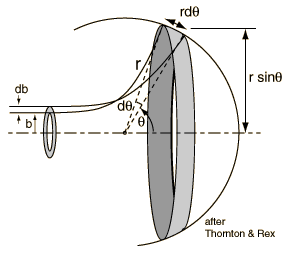
\includegraphics[width = 4 cm]{ruthcross.png}
  \begin{center}
  \caption{Depiction of a classical particle being scattered by the Coulomb Force.}[\footnotesize{``Scattering Cross Section.'' HyperPhysics. N.p., n.d. Web. 12 Mar. 2015.}]
  \label{ScatteringTheory}
  \end{center}
\end{figure}

Melissinos begins with the trajectory equation

\begin{equation}
  \frac{d^{2}u}{d\theta^{2}}+u=-\frac{Z_{1}Z_{2}e^{2}}{4\pi\epsilon_{0}mv_{0}^{2}b^{2} } = - \kappa
  \label{StartDerivation}
\end{equation}

with $u={1 \over r}$, $v_0$ as the velocity of the incoming particle at infinity (the velocity of the particle with no interaction with the nucleus), and $b$ as the impact parameter. 

The general solution to Equation~\ref{StartDerivation} is 

\begin{equation}
u=u_{0}\cos(\theta-\theta_{0})-\kappa
\label{adsf}
\end{equation} 
where the boundary condition is $u\to 0 \quad$ and $r\sin\theta\to b \quad(\theta\to\pi)$ 

The deflection angle $\theta$ can be found by solving $r \to \inf$ as $\theta=2\theta_{0}-\pi=2\arctan b\kappa=2\arctan\frac{Z_{1}Z_{2}e^{2}}{4\pi\epsilon_{0}mv_{0}^{2}b}$, where $\theta_{0}=\frac{\pi}{2}+\arctan b\kappa$. With some manipulation, we get 

\begin{equation}
b=\frac{Z_{1}Z_{2}e^{2}}{4\pi\epsilon_{0}mv_{0}^{2}}\cot\frac{\theta}{2}
\label{ImpactParameter}
\end{equation}

Furthermore, with a radially symmetric potential, which Equation~\ref{Discrete Coulomb} is, the differential cross section is just 

\begin{equation}
\frac{d\sigma}{d\Omega} = \frac{b}{\sin{\theta}} \left|\frac{db}{d\theta}\right|
\label{EndDerivation}
\end{equation}

By combining Equation~\ref{ImpactParameter} and Equation~\ref{EndDerivation}, we arrive at

\begin{equation}
  \frac{d\sigma}{d\Omega}=\left  (\frac{Z_1Z_2e^2}{16E \pi \epsilon_0} \right )^2\sin^{-4}{\frac{\theta}{2}}
  \label{DifferentialCrossSection}
\end{equation}    

where $E = \frac{1}{2} m v_0^{2}$. (Equations (3) - (6) are from Wikipedia, using the ``Inspect Element'' functionality to get the LaTeX).

In our experiment, we already have $Z_2$, the atomic number of the alpha particle, and we control the angle $\theta$ of the detector. To find $Z_1$ in Equation~\ref{DifferentialCrossSection}, we must find $\frac{d\sigma}{d\Omega}$, which can be determined by finding the solid angle of the detector aperture and the number of detected particles in an interval of time as a function of angle. This relationship, in Reference~\cite{Melissinos}, can be found in the following equation

\begin{equation}
  I_s = I_0 N \frac{d\sigma}{d\Omega} d\Omega
  \label{NumberOfAlphasScattered}
\end{equation}   

where $I_s$ is the counting rate of scattered atoms at a certain angle, $I_0$ is the incident scattering rate, $N$ is the area density of gold foil, and $d\Omega$ is the solid angle of the detector. 

By combining the above two equations and plotting the log of the $\sin^{-4}$ term on the x-axis against the log of the differential cross section, $\frac{d\sigma}{d\Omega}$, we can use the slope of that line to find the charge through this relationship

\begin{equation}
\left  (\frac{Z_1Z_2e^2}{16E \pi \epsilon_0} \right )^2 = 10^{m} cm^{-2}
\label{PrecedingTerm}
\end{equation}

where m is the slope of the line. 

\subsection{Energy Loss}

In this experiment, alpha particles lose energy for two main reasons: interactions with the electron clouds and the passing through the wall of the gun. There are also other reasons for energy loss: Cherenkov radiation, bremsstrahlung, and inelastic nuclear interactions. Before energy loss, the energies of the particles are broken up roughly into three categories: The energies of emitted alpha particles are 5.49 MeV (86\%), 5.44 MeV (13\%), and 5.39 MeV (1.3\%). Due to the brevity of time to conduct and do analysis of this experiment, we will forgo a detailed derivation of the energy loss from these effects. Instead, we will take the average energies of the alpha particles to be 3.77 MeV when they reach the detector. One can go more depth into the details of the energy loss by looking in Reference~\cite{Comfort}.

%%%%%%%%%%%%%%%%%%%%%%%%%%%%%%%%%%%%%%%%%%%%%%%%%%%%%%%%%%%%%%%%%%%%%%%%%%%%%
\section{Equipment and Setup}

\begin{figure}[htp]
  \begin{center}
    \subfigure[Table Set-up]{\label{Table}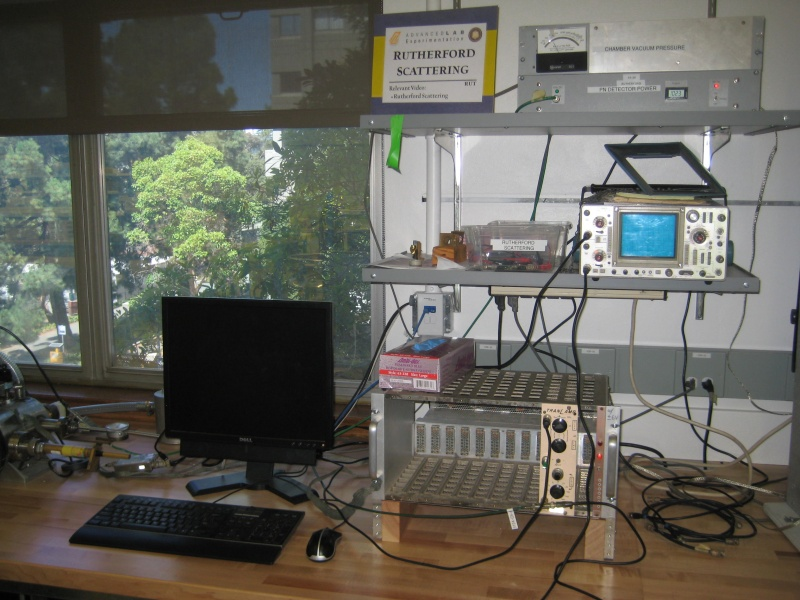
\includegraphics[width=4 cm]{RUT1.jpg}}
    \subfigure[Vacuum Valve]{\label{Valve}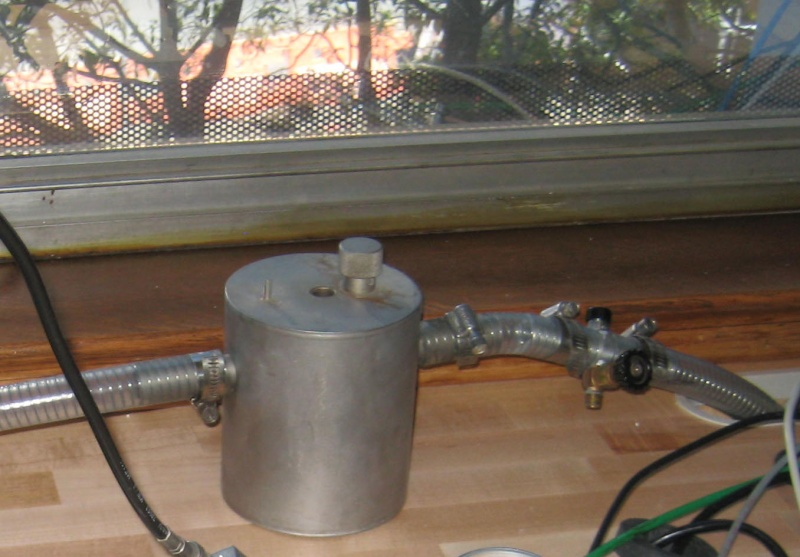
\includegraphics[width=4.3 cm]{RUT2.jpg}} \\
    \subfigure[Scattering Chamber]{\label{Chamber}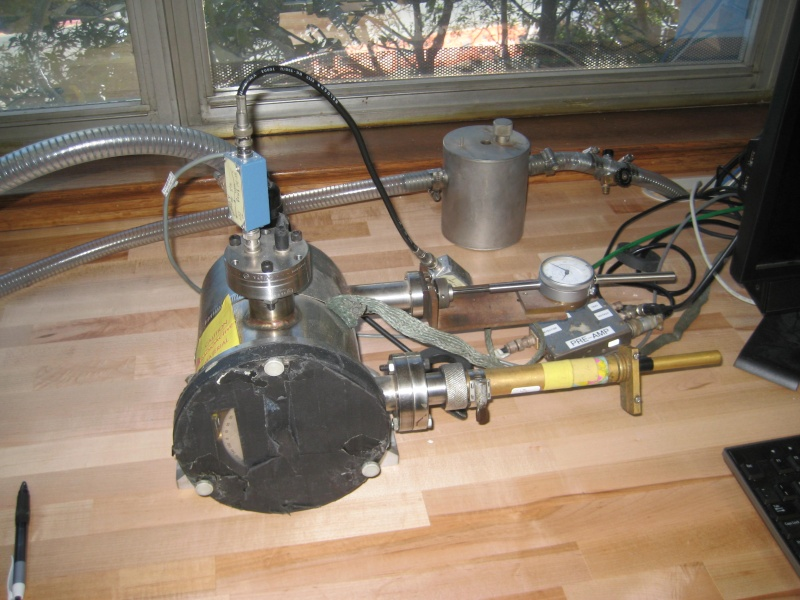
\includegraphics[width=5 cm]{RUT3.jpg}}
  \end{center}
  \caption{Rutherford Experiment Setup at UC Berkeley}[\footnotesize{``Rutherford Scattering.'' - Physics 111-Lab Wiki. UC Berkeley, n.d. Web. 13 Mar. 2015.}]
  \label{ThreeFigs}
\end{figure}

\begin{enumerate}
\item Vacuum Chamber with an adjustable detector and corresponding angle measure to measure the angle between the detector and the axis of the alpha gun. Our detector is a Silicon PN-junction with about 250 microns of gold on it. It has a bias of 50 volts at 4 microamps with a diameter of 0.75 inches. The detector receives its power through a voltage divider to get 50 volts from the 100 volt power supply in the rack
\item An alpha particle source. In our experiment, we used Americium 241. 
\item A gun in which the alpha particle is placed with an adjustable aperture size. Our gun was placed 7.8 cm away from the detector. 
\item Double layers of gold leaf foils that can be mounted in front the alpha gun.
\item A vacuum pump. Our chamber was set to a pressure of 80 Torr. 
\item An oscilloscope to detect energy from the alpha gun. 
\item A data taking software. In our experiment, we used a pre-coded LabVIEW program called PHA-5124. This allowed us to measure the energies, counts, and set the gain of energies of the alpha particles that interacts with the detector. 
\item Pre-amp
\item Tran-L-Amp
\end{enumerate}

All equipment can be seen in the figures: Figure~\ref{ThreeFigs}, Figure~\ref{Diagram}, and Figure~\ref{OutsideDiagram}.

\begin{figure}[h]
  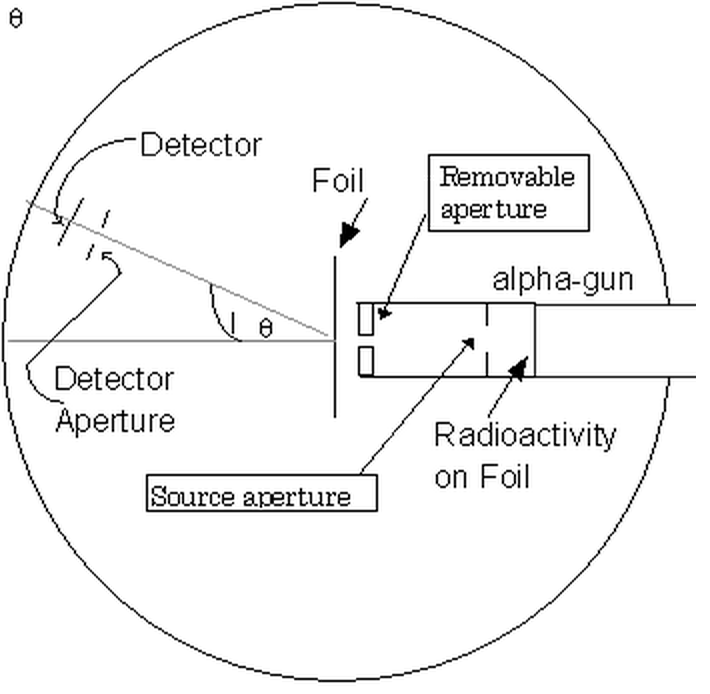
\includegraphics[width = 3.5 cm]{Diagram.png}
  \begin{center}
  \caption{Inside the vacuum chamber}[\footnotesize{``Rutherford Scattering.'' - Physics 111-Lab Wiki. UC Berkeley, n.d. Web. 13 Mar. 2015.}]
  \label{Diagram}
  \end{center}
\end{figure}

\begin{figure}[h]
  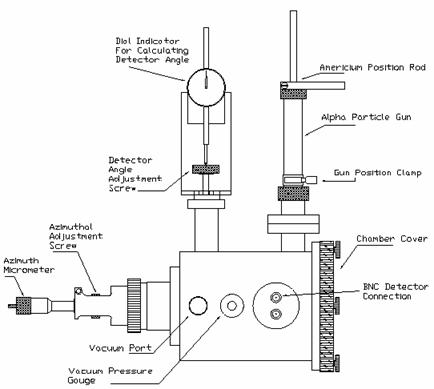
\includegraphics[width = 5 cm]{Diagram2.jpg}
  \begin{center}
  \caption{Outside the vacuum chamber}[\footnotesize{``Rutherford Scattering.'' - Physics 111-Lab Wiki. UC Berkeley, n.d. Web. 13 Mar. 2015.}]
  \label{OutsideDiagram}
  \end{center}
\end{figure}

\subsection{Taking Measurements}

For our experiment, we first created a vacuum in the chamber. Then we adjusted the Tran-L-Amp to where we set the DIFF to 1.0, INT to 0.05, Coarse Gain to 100, Vennier Gain to  5.9 microseconds, and the FINE GAIN at 1.75. Finally, with the detector at 0 degrees, we make sure that the detector is receiving a signal that displays on the oscilloscope. An example of this signal is in Figure~\ref{Scope}.

\begin{figure}[h]
  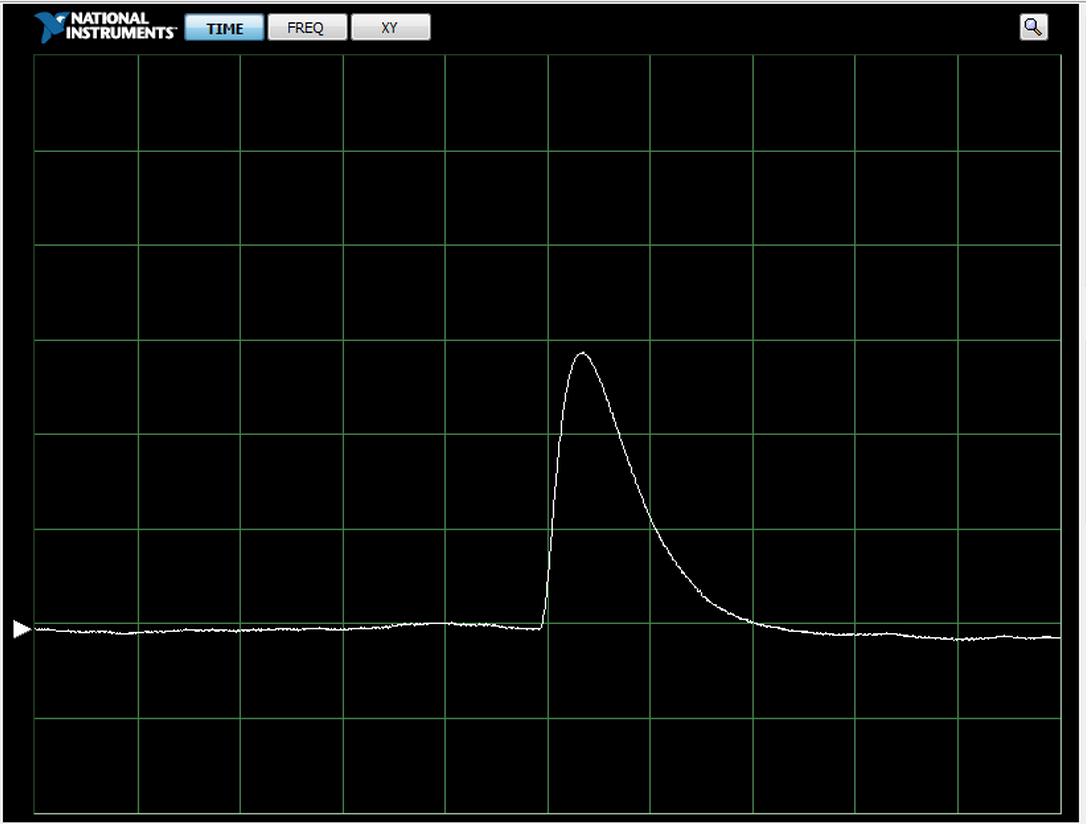
\includegraphics[width = 3 cm]{Scope.png}
  \begin{center}
  \caption{The feed into the scope}[\footnotesize{``Rutherford Scattering.'' - Physics 111-Lab Wiki. UC Berkeley, n.d. Web. 13 Mar. 2015.}]
  \label{Scope}
  \end{center}
\end{figure}

\clearpage

\begin{figure*}[t]
  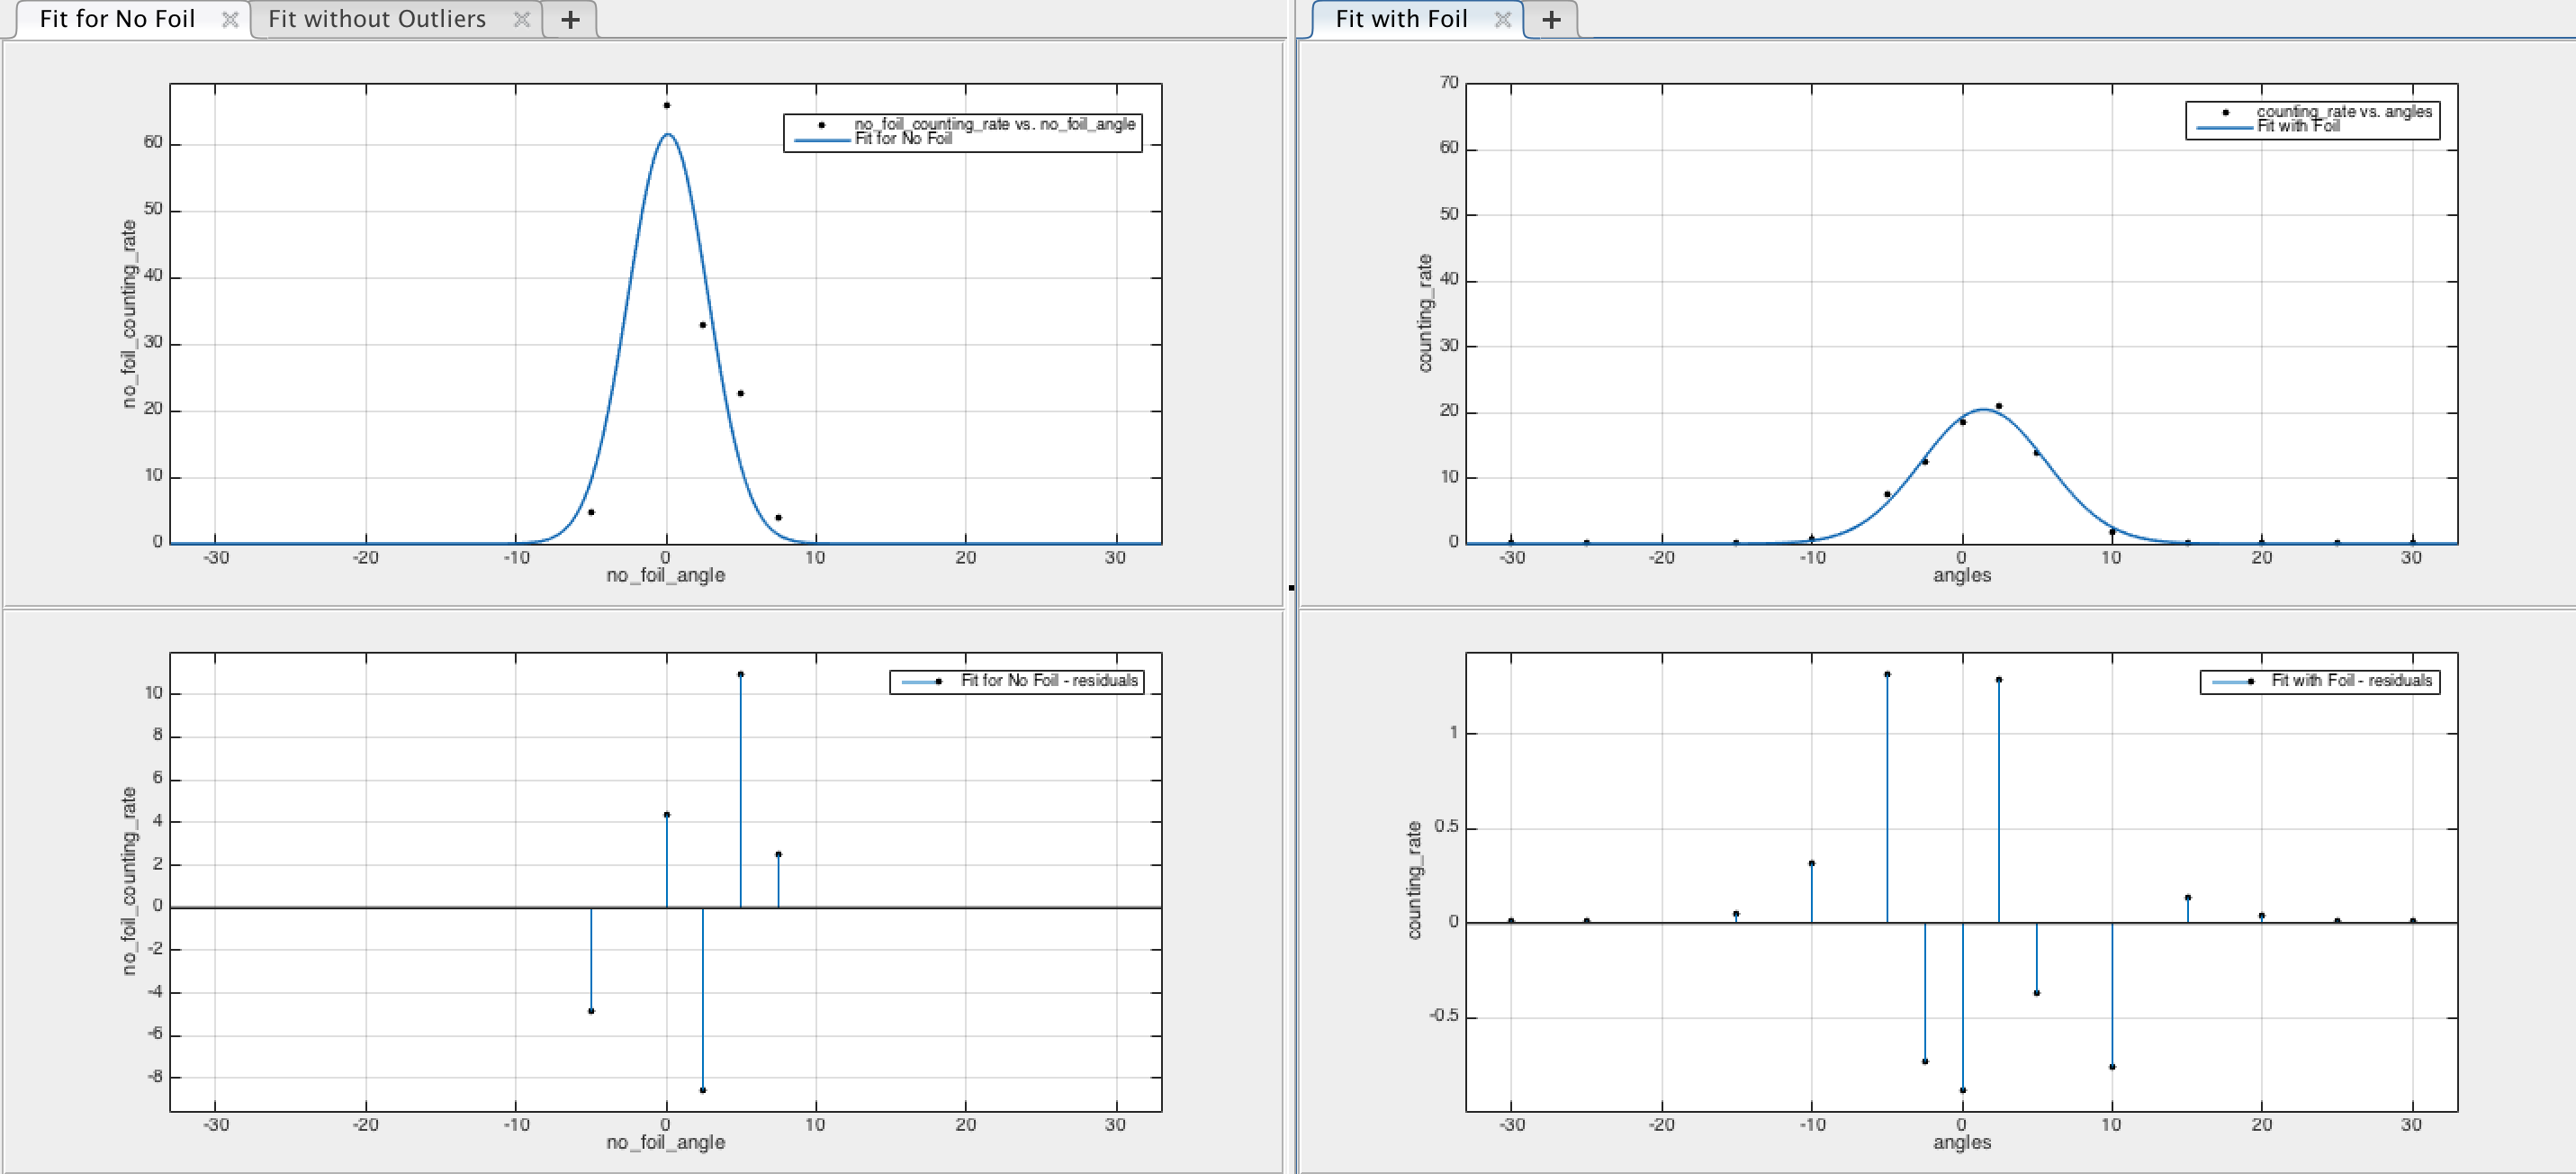
\includegraphics[width=\textwidth]{CombinedGraphs.png}
  \begin{center}
  \caption{Gaussian Fit of angle vs. counting rates for both no foil and with foil}
  \label{Combined}
  \end{center}
\end{figure*}

\section{Measurements and Analysis}


When we took measurements, we first took measurements of the intensity of the alpha gun itself, then the angle dependence of the alpha particles without any gold foil, and then finally we included the gold foil and found the angle dependence. 

In Table~\ref{PointBlank} we see the counting rate of the gun at point blank. This is much greater than the maximum counting rate of gun at its default position of 7.8 cm. With that distance, the maximum counting rates were much less than the point blank counting rate. However, we can see from Table~\ref{NoFoilTable} that when the point rates of the angles are summed up, we get near the total counts when we have the gun at point blank. This indicates to us that the alpha particle beam is not emitting straight out of the gun; instead, it had an angular dependence. In the theory we discussed energy loss due to collisions with the walls of the gun. In Table~\ref{Energies}, however, we see that at an angle of 5 degrees, the mean energy is roughly the same for 0 degrees and point blank. What is probably happening is that the alpha particle is colliding many times within the gun, and on average, alpha particles are colliding an equal amount of times before exiting the gun. Therefore, the average energy leaving the gun is angle independent. 


We also noticed that in the case of no foil, the counts of alpha particles drops of very quickly past 5 and -5 degrees (see the left plot in Figure~\ref{Combined}). This means that when we insert the gold foil, counts that we receive past 10 and -10 degrees are most likely due to alpha particles scattering off the gold foil.

\begin{table}[h]
  \begin{tabular}{|l|l|}
  \hline 
  Measurement & Count Rate (counts/s)                \\ \hline \hline
  Point Blank & 104.84 $\pm$ 10.39                        \\
  No Foil, 7.8 cm away from detector & 65.86 (Max Value)    \\
  With Foil, 7.8 cm away from detector & 40.76 (Max Value)  \\ \hline         
  \end{tabular}
  \caption{Counting Rate for 3 situations, Point Blank, no foil, and with foil.[\footnotesize{Throughout this paper, the $\pm$ symbol will be used to denote 1 standard deviation of error, while the parentheses notation (NUMBER, NUMBER) will denote 95$\%$ confidence bounds.}]}
  \label{PointBlank}
\end{table}

\begin{figure*}[t]
  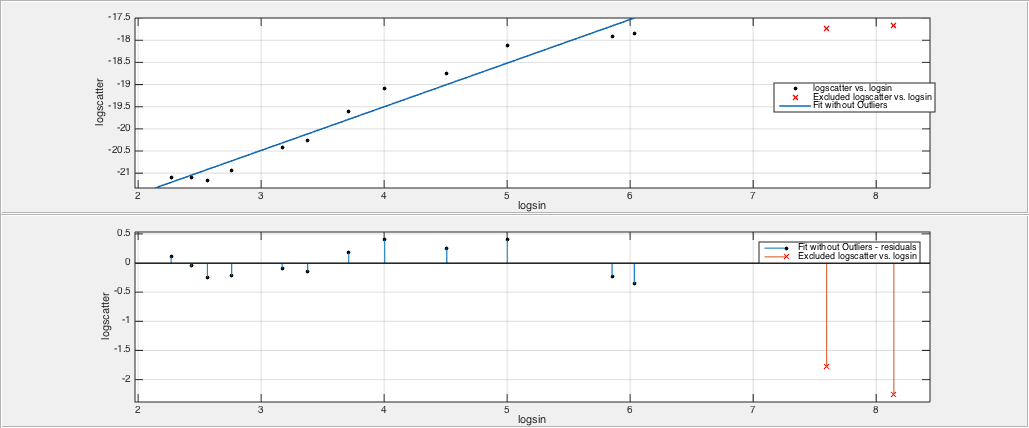
\includegraphics[width=\textwidth]{FitforScatteringCrossSection.png}
  \begin{center}
  \caption{Scattering Cross Section vs. $ \sin(\frac{\theta}{2})^{-4}$, where ``logscatter'' = $\log{d \sigma / d \Omega}$ and ``logsin'' = $\log{\sin(\frac{\theta}{2})^{-4}}$. The fit has an R$^2$ value of 0.9605. We discuss the removal of certain points in the Error Analysis section of this paper.}
  \label{FitforScatteringCrossSection}
  \end{center}
\end{figure*}

\begin{table}[h]
  \begin{tabular}{|l|l|}
  \hline
  No Foil Angle & Counting Rate (counts/s) \\ \hline \hline
  -5            & 4.70                          \\
  0             & 65.86                         \\
  2.5           & 32.96                         \\
  5             & 22.54                         \\
  7.5           & 3.863333333                   \\ \hline
  \end{tabular}
  \caption{Point blank counting rate as a function of angle. We were not able to determine error for these values due to our small sample size.}
  \label{NoFoilTable}
\end{table}

\begin{table}[h]
  \begin{tabular}{|l|l|}
  \hline
  Angle (Degrees) with No Foil & Energy    \\ \hline \hline
  0               & 4.75 $\pm$ 0.74        \\
  5               & 4.74 $\pm$ 0.67        \\
  Point Blank     & 4.69 $\pm$ 0.94        \\ \hline
  \end{tabular}
  \caption{Average energy comparison between the energy of no-foil alpha particles and point-blank alpha particles.}
  \label{Energies}
\end{table}

Now that we've seen how the alpha particles scatter without the gold foil, we can begin looking at the scattering with the gold foil in place. We fit the data to a Gaussian Distribution because the data points looked like they were following a Gaussian curve. Figure~\ref{Combined} shows a wider distribution for the angle, which confirms our theory that gold can scatter alpha particles beyond small angles. For the case of the foil, the standard deviation is 5.92 degrees, which is 57\% larger than 3.76 degrees the standard deviation for no foil. Although there is a difference, this degree of difference is not unexpected, due to the tiny size of the gold nucleus, which is on the order of femtometers. We ought to be seeing a wider spread for the case of the gold foil, but not an absurdly large difference since the small size of the nucleus means that most alpha particles will be deflected a small amount. Large angle deflections would be indicative of alpha particles either coming very close (distance $<<$ the size of a gold atom) to one or multiple gold nuclei. 

Another observation that we made was that the counting rate with the gold foil is less than the counting rate for the case without gold foil. The maximum counting rate near the 0 angle position, according to the Gaussian Fit, was 41 fewer counts/second in the case of the gold foil. This difference is expected due to alpha particles getting scattered outwards from the 0 angle. 

\begin{table}[h] 
  \begin{tabular}{|l|l|l|}
  \hline
  Measurement & Zero-Position (Degrees) & Peak Mag. (counts/s) \\ \hline \hline
  No Foil     & 0.1401 $\pm$ 3.761  & 61.54  (17.1, 106)   \\ 
  With Foil   & 1.45 $\pm$ 5.92 & 20.47  (19.32, 21.61) \\ \hline     
  \end{tabular}
  \caption{Gaussian Fit of Counting Rate Data (with 95$\%$ confidence bounds)[\footnotesize{Note: Our plot with gold foil shows large 95$\%$ confidence intervals for the plot for no foil. We will discuss these discrepancies in the error section of our paper.}]}
  \label{ZeroPosition}
\end{table}

With these plots, we can begin to calculate the atomic number of the gold atom. We first corrected the angles by subtracting each angle by 0.7366 degrees and then calculated $ \sin(\frac{\theta}{2})^{-4}$ of those angles. Those values are the x-values of Figure~\ref{FitforScatteringCrossSection}. By using the values of Table~\ref{Values} in Equation~\ref{NumberOfAlphasScattered} and counting rate data that we measured, we found the Differential Cross Section, which is the y-axis of Figure~\ref{FitforScatteringCrossSection}. The resulting best-fit value for term is $10^{-23.66}$ cm$^{-2}$. With a bit of algebra, we found that $Z_1$ yields 99.77, which is a 26.3$\%$ error from the actual value of 79. Additionally, our 95$\%$ confidence interval (-24, -22.88) gives us a confidence interval for the atomic number between (52.36, 190.12), which encloses 79 as the atomic number. Therefore, our results are close to the theory.

\begin{table}[h]
  \begin{tabular}{|l|l|}
  \hline 
  Variable                         & Value               \\ \hline \hline 
  Incident Counting Rate           & 104.84 counts/sec   \\
  Detector Solid Angle             & 0.0060 sr           \\
  Area Density of Gold Foil        & $1.57 * 10^{19}$ atoms/cm$^2$ \\
  Atomic Number of Alpha Particle  & 2                   \\
  Average Energy of Alpha Particle & 3.77 MeV        \\ \hline
  \end{tabular}
  \caption{Values for Equation ~\ref{NumberOfAlphasScattered}}
  \label{Values}
\end{table}

\begin{table}[h]
\begin{tabular}{|l|l|l|}
\hline
Parameter  & Value (without Outliers) & Value (with Outliers)   \\ \hline \hline
m               & 0.9846  (0.8439, 1.125)   & 0.6838  (0.5112, 0.8565)    \\
b               & -23.44  (-24, -22.88)     &  -22.41  (-23.23, -21.59) \\ \hline
\end{tabular}
\caption{Parameters for the equation $y=mx+b$ with 95$\%$ confidence intervals, where y is the log of the scattering cross section, mx is the $\sin$ term, and b is the log of the term preceding the $\sin$ term in Equation~\ref{DifferentialCrossSection}. $10^b$ is in units of cm$^{-2}$ and m is dimensionless. Figure~\ref{FitforScatteringCrossSection} corresponds to these fit values.}
\label{CurveFitValues}
\end{table}

\section{Error Discussion}

\begin{figure*}[tt]
  \begin{center}
    \subfigure[Scattering with Foil at 0 degrees]{\label{0DegreeNoise}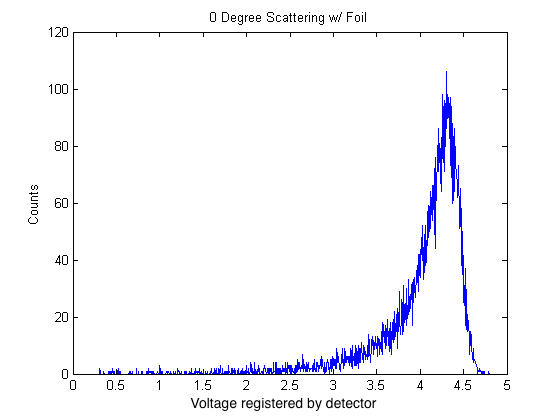
\includegraphics[width=7 cm]{0degreeScatteringFoil.png}}
    \subfigure[Scattering with Foil at 30 degrees]{\label{30DegreeNoise}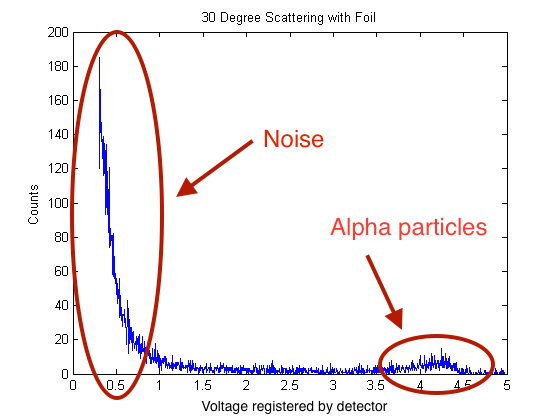
\includegraphics[width=7 cm]{30degreeScatteringFoil.png}} \\
  \end{center}
  \caption{Comparison between the registered voltage of counts at 0 degrees and 30 degrees.}
  \label{Noise}
\end{figure*}

\begin{figure*}[tt]
  \begin{center}
    \subfigure[Error in Angle with Foil]{\label{ErrorAngleFoil}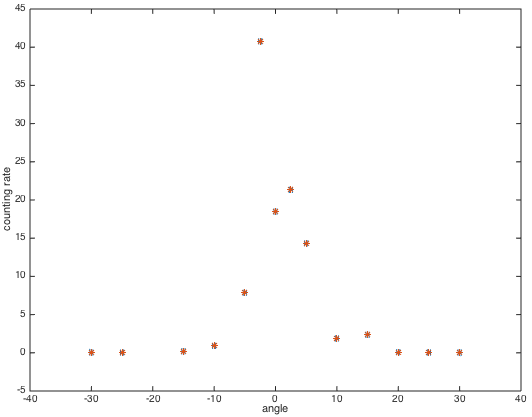
\includegraphics[width=6 cm]{errorfoil.png}}
    \subfigure[Error in Angle without Foil]{\label{ErrorAngleNoFoil}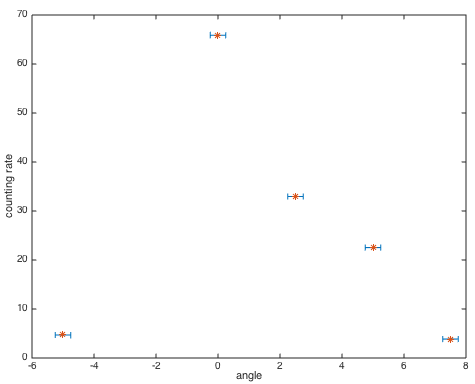
\includegraphics[width=6 cm]{errornofoil.png}} \\
  \end{center}
  \caption{Plots with error bars on the analog angle error.}
  \label{AngleError}
\end{figure*}

While this experiment has errors due to analog angle measurements and analog solid angle measurements, this experiment's biggest area of error was due to the small sample of data we took. For example, in Tables~\ref{ZeroPosition} and \ref{ZeroPosition2}, the confidence intervals for those values are large. Since we had only 9 days to do the experiment, that meant that we only had 8 nights to run longer runs. These longer runs were made for large angles because the counting rate for large angles are so small. For instance, for angles of magnitude 20 degrees or larger, the counting rate was on the order of 1 count every 100 seconds. This limited the amount of large-angle data sets that we were able to take. 

On the other hand, the curve fit values in Table~\ref{CurveFitValues} have relatively smaller confidence intervals due to a larger sample size. If we were given more time to conduct the experiment, we would have more data and have smaller confidence intervals for our Gaussians and for the Linear Fit.

Another area of Error was in our linear fit. From the theory we expected the log log plot to yield a slope of 1, yet with the outliers we calculated a slope of 0.6838 with a confidence interval of (0.5112, 0.8565). We determined that the two points to remove would be the points with the largest $\log{\sin(\frac{\theta}{2})^{-4}}$ value because at that level, the corresponding $\theta$ is very small. Therefore, when small angles are taken to the power of -4, any errors get incredibly magnified. To confirm this, we removed the outliers and our slope changed from 0.68 to 0.98, which is much closer to the theory. 

Our last area of error was in the low energy regions. In Figure~\ref{30DegreeNoise}, we see a very large spike in the plot with voltages under 1 V. This noise gets amplified over time because for 30 degrees, our data sampling time was 216000 seconds, whereas for 0 degrees it was 600 seconds. This allowed noise to build up over time. By looking at Figure~\ref{0DegreeNoise}, we can see that the noise scales correctly to Figure~\ref{30DegreeNoise}, given the increase in time scale. We believe that these counts are noise from electrical fluctuations from nearby equipment, background radiation, and/or because our chamber was not a perfect vacuum. To correct for this, we set the threshold for a true registered alpha particle count to be any hit over 2 V.  

\section{Conclusion}

Rutherford Scattering was a groundbreaking experiment that showed the world that the atom has a concentrated volume of positive charge in the middle of the atom. By using a vacuum chamber, a radioactive source, gold foil, and a detector, we were able to measure the amount of alpha particles detected per second as a function of angle. Then by knowing how the scattering cross section varies as a function of angle, we were able to plot the log of both parameters and find the intercept value, which corresponded to the atomic number of gold. 

First, we found the angular dependence of the alpha particles without any gold foil in place. In theory, there should be a narrower Gaussian with no gold foil, since there are no gold atoms in the alpha particles' trajectories to deflect them. We were able to see that with no gold foil, the spread of the Gaussian was smaller than with the gold foil, which confirms the theory. 

Finally, when we insert the gold foil into place and begin taking data of counts at different angles, we see very small but non-zero counts of alpha particles at angles from 20 to 30 degrees. By calculating Equation~\ref{NumberOfAlphasScattered} with the counting rates and values in Table~\ref{Values}, we were able to find the differential cross section. This differential cross sectino is crucial because it is the left hand side for Equation~\ref{DifferentialCrossSection}. Then we plotted the angular dependence of the differential cross section. We arrived at an atomic number of 99.77 with a 95$\%$ confidence interval of (52.36, 190.12). This is near the theoretical value of 79. 

Although our value for the atomic number is close to the theoretical value, there is still a lot of work that can be done. We were restricted to a short time frame, which limited the amount of data that we could take. Therefore, given more time, we would have taken more data to get better fits and smaller confidence intervals. Also given the equipment, we would have taken data on background radiation to see how much of our actual data is noise and how much is due to the alpha particles. 

All in all, this experiment is a great introduction into data analysis and atomic structure. It invites further experimentation to get better fits, investigate outliers (for example, points near 0 degrees where errors get extremely magnified by the power to -4), and even probe the size of a gold nucleus by looking for scattering angles greater than 30 degrees. 


%%%%%%%%%%%%%%%%%%%%%%%%%%%%%%%%%%%%%%%%%%%%%%%%%%%%%%%%%%%%%%%%%%%%%%%%%
% Place all of the references you used to write this paper in a file
% with the same name as following the \bibliography command
%%%%%%%%%%%%%%%%%%%%%%%%%%%%%%%%%%%%%%%%%%%%%%%%%%%%%%%%%%%%%%%%%%%%%%%%%


% %%%%%%%%%%%%%%%%%%%%%%%%%%%%%%%%%%%%%%%%%%%%%%%%%%%%%%%%%%%%%%%%%%%%%%%%%%%%%
\begin{acknowledgments} I acknowledge my lab partner Tanooj Shah for taking data for the both of us when I was ill. I also want to acknowledge Prof Stamper-Kurn for asking challenging questions but ultimately pushing Tanooj and me to truly understand the lab.
\end{acknowledgments}

\begin{thebibliography}{9}

\bibitem{Melissinos}
  A.C. Melissinos, \emph{Experiments in Modern Physics}, Rutherford Scattering, Academic Press Inc. pg. 231-252, 1966

\bibitem{youtube}
  Sumner Davis, \emph{Rutherford Scattering}, https://youtu.be/xHzzXiMEmaU, March 7, 2012

\bibitem{Wikipedia}
  Various Pages for Images, http://wikipedia.com/, March, 2015

\bibitem{website}
  Physics 111 ADV Lab, \emph{Rutherford Scattering}, http://advancedlab.berkeley.edu/, February, 2015

\bibitem{Comfort}
J.R. Comfort, et al., ``Energy Loss and Straggling of α Particles in Metal Foils'', Phys. Rev. 150, 249 (1966)

\end{thebibliography}


\end{document}
